\chapter{Drei Raumrichtungen und eine Zeit: Welche Bedingungen bleiben?}
\label{ch:shadow-dimension}
\begin{bild}{Dimension ist die Antwort auf eine Frage}
Eine Ameise auf einer dünnen Schnur kann entlang einer Richtung laufen. Auf einem Blatt kann sie außerdem ausweichen. In einem Zimmer kann sie auch über ein Hindernis hinweg. Eine Dimension zählt solche unabhängigen Möglichkeiten. Die Zahl der inneren Zustandskomponenten oder der Knöpfe eines Geräts ist etwas anderes.
\end{bild}

Unsere gewöhnliche makroskopische Beschreibung benötigt drei Raumkoordinaten und eine Zeitkoordinate. Das ist die Zielstruktur im beobachteten Gültigkeitsbereich, kein Beweis, dass bei jeder denkbaren Skala ausschließlich vier kontinuierliche Koordinaten fundamental existieren. Ein $E_8$-Rang 8, vier interne Zustände und eine dreidimensionale räumliche Ausbreitung zählen jeweils andere Dinge.

\section{Drei unterschiedliche Hinweise führen zur Zahl drei}
Ein traceloses hermitesches $2\times2$-Objekt hat genau drei reelle Komponenten:
\[
 h=x\sigma_x+y\sigma_y+z\sigma_z.
\]
Ergänzt man $tI$, ergibt die Determinante
\[
 \det(tI+h)=t^2-x^2-y^2-z^2.
\]
Der positive Kegel erfüllt $t\geq\sqrt{x^2+y^2+z^2}$. Das ist die präzise Lorentz-Brücke aus dem Ursprungsteil. Sie zeigt eine passende lokale algebraische Form. Noch fehlen ihre Interpretation als Ereignisse, die Verklebung zu einer Raumzeit und die richtige Dynamik.

Ein zweiter Hinweis ist ein generisches Zweibandmodell $H(k)=d_0(k)I+\sum_{a=1}^3d_a(k)\sigma_a$. Eine Entartung benötigt drei Gleichungen $d_1=d_2=d_3=0$. In einem dreidimensionalen Impulsraum kann sie deshalb isoliert und bei geeigneter topologischer Ladung stabil sein. Die Wahl eines Zweibandsektors und eines geeigneten kontinuierlichen Impulsraums wird dabei schon vorausgesetzt. Andere Symmetrien können diese Zählung verändern. \src{E11, E12}

Ein dritter Hinweis kommt aus Ausbreitung. Wenn eine Anregung bei langen Wellen in drei unabhängigen Richtungen propagiert, sollten Zustandsdichte, Wärmeausbreitung und Fernkorrelationen dieselbe Dimension anzeigen. Erst die Übereinstimmung dieser operational verschiedenen Bestimmungen wäre ein stärkerer Befund als eine einzelne passende Matrix.

\section{Eine neue Gegenprobe am Clebsch-Vorschlag}
Für einen Graph-Laplaceoperator $L$ definieren wir die mittlere Rückkehrfunktion und eine skalenabhängige Dimension durch
\begin{equation}
 P(\tau)=\frac1{|V|}\Tr e^{-\tau L},\qquad
 d_s(\tau)=-2\frac{d\log P(\tau)}{d\log\tau}.
\end{equation}
Auf einem großen regelmäßigen dreidimensionalen Gitter entsteht zwischen der Gitter- und der endlichen Systemskala ein Bereich mit $P(\tau)\sim\tau^{-3/2}$, also $d_s\approx3$. Bei einem endlichen zusammenhängenden Graphen geht $d_s$ sowohl für sehr kleine als auch sehr große $\tau$ gegen null. Deshalb ist ein \emph{ausgedehnter Zwischenbereich mit kontrollierter Vergrößerung} relevant.

Der Clebsch-Graph besitzt für $L=5I-A$ die Eigenwerte $0,4,8$ mit Vielfachheiten $1,10,5$. Somit gilt exakt
\[
 P_{\mathrm{Cl}}(\tau)=\frac{1+10e^{-4\tau}+5e^{-8\tau}}{16}.
\]
Eine einzelne solche Kurve liefert keine makroskopische dreidimensionale Geometrie. Die folgende Vergleichsrechnung zeigt, wie eine richtige Größenfamilie aussehen müsste.

\begin{figure}[H]\centering
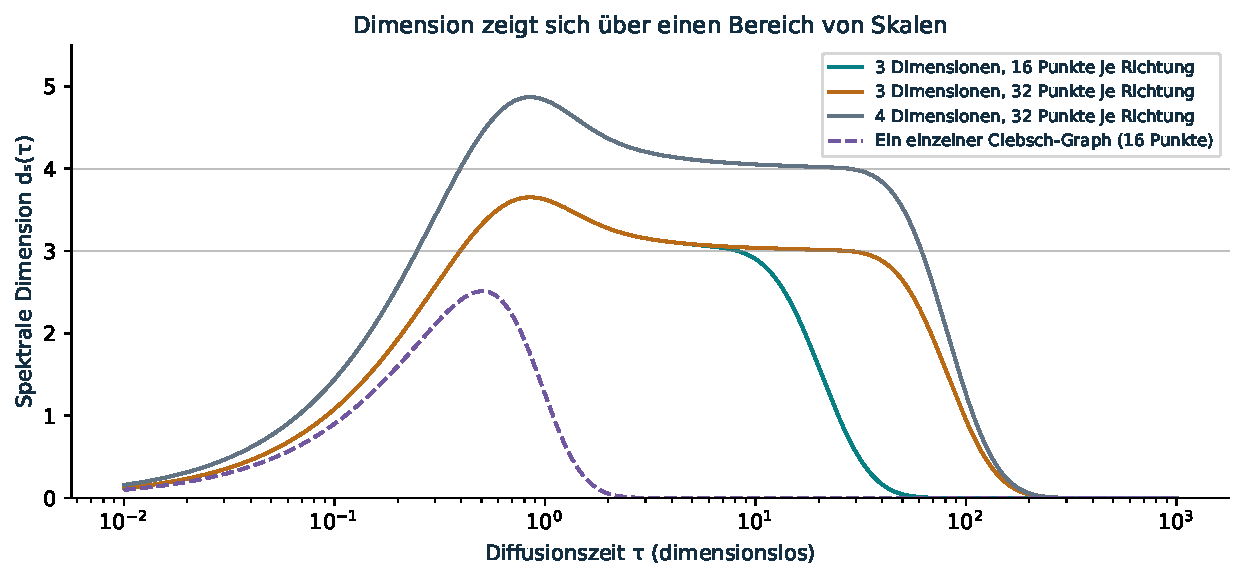
\includegraphics[width=\linewidth]{figures/shadow_dimension.pdf}
\caption{Eigene Wärmeausbreitungsrechnung. Regelmäßige periodische Gitter zeigen einen Bereich nahe ihrer eingesetzten Dimension; der Einzel-Clebsch-Graph besitzt keine daraus abgeleitete dreidimensionale Skalenfamilie. Der vierdimensionale Vergleich ist euklidisch und zählt keine Lorentz-Zeit.}
\end{figure}

Die Gitter sind hier bewusst eingesetzte Kontrollbeispiele. Ihre Dimension wurde nicht aus TFPT gewonnen. Ein nächster nativer Test müsste eine \emph{aus derselben Quelle erzeugte} wachsende Zellfamilie, deren Kopplungen und die passende Diffusions- oder Anregungsdynamik verwenden. Ein punktuelles Kreuzen von $d_s=3$ genügt nicht.

\section{Eine Zeitrichtung ist mehr als ein weiterer Zahlenplatz}
In einer gewöhnlichen hyperbolischen Wellengleichung werden lokale Anfangsdaten auf einer räumlichen Fläche vorgegeben und entlang einer ausgezeichneten Zeitrichtung entwickelt. Mehrere Zeitkoordinaten verändern das Anfangswertproblem grundlegend. Unter zusätzlichen nichtlokalen Beschränkungen existieren dennoch wohldefinierte Mehrzeit-Probleme; ein pauschaler Unmöglichkeitssatz wäre falsch. \src{F14}

Für unseren Ansatz entsteht deshalb eine konkrete Auswahlaufgabe: Aus der Quelle müssen ein geeigneter Kausalkegel, erlaubte Anfangsdaten, stabile Evolution und eine konsistente lokale Energiebedingung hervorgehen. Der innere modulare Fluss einer Dichtematrix, der arithmetische $\log n$-Fluss und die im Labor gemessene Zeit sind zunächst drei verschiedene Konstruktionen. Ihre Gleichsetzung braucht einen eigenen Satz oder ein operationales Vergleichsexperiment.

\section{Was Stabilität zusätzlich einschränkt}
Ein elementares mechanisches Beispiel illustriert die Rolle von Constraints. Nimmt man in $d>2$ Raumdimensionen eine Newtonsche Punktkraft mit Gaußgesetz an, lautet das effektive Radialpotential
\[
 V_{\mathrm{eff}}(r)=\frac{\ell^2}{2mr^2}-\frac{k}{(d-2)r^{d-2}}.
\]
An einer Kreisbahn ergibt sich
\[
 V_{\mathrm{eff}}''(r_0)=\frac{(4-d)\ell^2}{mr_0^4}.
\]
Unter diesen Voraussetzungen sind solche Kreisbahnen bei $d=3$ stabil, bei $d>4$ instabil und bei $d=4$ in dieser Näherung marginal. Das ist eine eigene ausgeschriebene Modellrechnung, kein universeller Dimensionsbeweis: $d=2$ verwendet ein logarithmisches Potential; andere Kräfte und Dynamiken verändern das Ergebnis.

\textbf{Die gemeinsame Schlussfolgerung:} Drei Raumdimensionen werden plausibler, wenn lokale Matrixstruktur, stabile Anregungen, Ausbreitung und makroskopische Stabilität zusammenpassen. Keine der einzelnen Beobachtungen erzwingt bereits die ganze Auswahl. Der noch fehlende Schritt liegt in ihrer gemeinsamen Herkunft und im kontrollierten Skalenübergang.
